\documentclass{article}
\usepackage{graphicx}
\usepackage{sidecap}
\usepackage{fancyhdr}
\usepackage[absolute]{textpos}
\usepackage{listings}
\usepackage{amsmath}
\usepackage[utf8]{inputenc}
\usepackage[francais]{babel}
\usepackage{sistyle}
\usepackage{amsmath}
\usepackage{hyperref}
\usepackage{color}
\usepackage{adjustbox}
\usepackage{floatrow}
\usepackage{float}
\DeclareCaptionFont{Small}{\fontsize{9}{11}\selectfont}
\usepackage{wrapfig}
\usepackage[bottom]{footmisc}
\usepackage[dvipsnames]{xcolor}
\usepackage{caption}
\usepackage{float}
\usepackage{sidecap}
\usepackage{fancyhdr}
\usepackage{lscape}
\usepackage{cmap}
\usepackage[T1]{fontenc}   %Allow accent to be copy and pasted correctly
\usepackage[utf8]{inputenc}
\usepackage[francais]{babel}
\usepackage[absolute]{textpos}
\usepackage{url}
\usepackage{array}
%%\setlength{\parindent}{4em}
%%\setlength{\parskip}{1em}
\frenchbsetup{StandardItemLabels=true, CompactItemize=false, ReduceListSpacing=true}


\renewcommand{\thepage}{\arabic{page}}
\setcounter{page}{0}

\addto\captionsfrench{\renewcommand{\figurename}{Image}}


\usepackage[top=3cm , bottom=3cm, left=2cm , right=2cm]{geometry}


\makeatletter
\def\maketitle{%
  \null
  \thispagestyle{empty}%
  \vfill
  \begin{center}\leavevmode
    \normalfont
    
\includegraphics[width = 140mm]{./ulb.jpg}
    {\LARGE \@title\par}%
    \vskip 0.5cm
    {\Large \@author\par}%
    \vskip 0.5cm
    {\Large \@date\par}%
    %\includegraphics[width = 60mm]{/Users/nicolaspotie/Desktop/ulb2.jpg}
  \end{center}%
  \vfill
  \null
  \newpage
  }
\makeatother
\author{Nicolas Potie, Yann Sp\"ori\\ Master 2 en bioinformatique et modélisation}
\title{\\INFOH410:Summary}
\date{June 2017}

%partie concernant la gestion des entÍtes
\pagestyle{fancy}
\renewcommand\headrulewidth{1pt}
\fancyhead[L]{Nicolas Potie, Yann Sp\"ori}
\renewcommand\footrulewidth{1pt}
\fancyfoot[C]{\thepage}
%fin

\begin{document}
%\maketitle
%\tableofcontents
\pagebreak

Entrophy:\\
\[
E(S)=-p_{+}(log_2{p_{+}})-p_{-}(log_2{p_{-}})
\]
Information gain:\\
\[
G(s,a) = E(S)-\sum_{v \in Values(A)} \frac{|S_v|}{|S|}E(S_v)
\]
Gain Ratio:
\[
GR(S,A) = \frac{Gain(S,A)}{SplitInformation(S,A)}
\]
SplitInformation:
\[
SplitInformation(S,A) = - \sum_{i=1}^{c} \frac{|S_i|}{|S|} log_2 \frac{|S_i|}{|S|}
\]
Candidate elimination algo:
\begin{figure}[H]
%\begin{center}
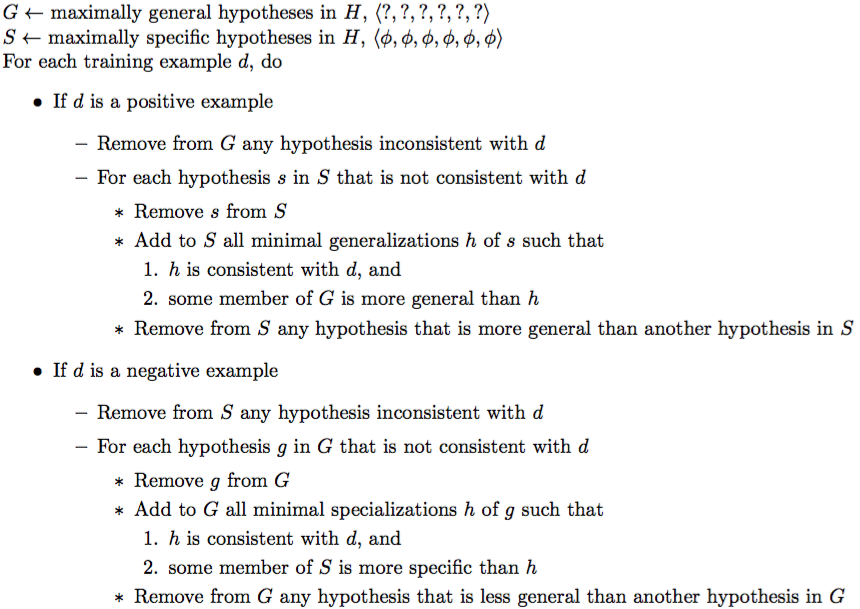
\includegraphics[width=.5\textwidth]{candidate_elim.png}
%\end{center}
\end{figure}
%\FloatBarrier
Euklidian Distance:\\
\[
d(P(x_1, y_1), P(x_2, y_2)) = \sqrt{(x_1-x_2)^2 + (y_1-y_2)^2}
\]
Manhattan Distance:\\
\[
d(P(x_1, y_1), P(x_2, y_2)) = |x_1-x_2| + |y_1-y_2|
\]
Q-learning:
\begin{figure}[H]
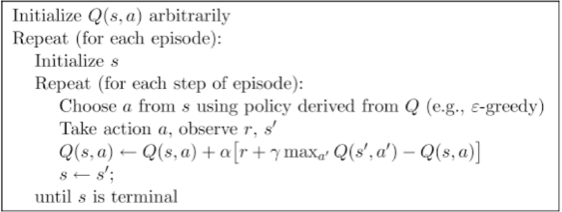
\includegraphics[width=.5\textwidth]{Q.png}
\end{figure}


\end{document}
